\chapter{Marco Teórico}

% En este capítulo, se presenta las principales tecnologías de detección en primer  plano del objeto en movimiento, descripción y extracción de características,  clasificación y reconocimiento del movimiento humano. Basado en el flujo óptico para la detección de objetos en movimiento. Como también la imagen de flujo de energía óptico para la detección de características de movimiento y se adoptaron redes neuronales convolucionales de región para elegir  características y reducir la dimensión. Luego, gracias al clasificador de máquina de vectores de soporte que puede ser entrenado y utilizado para clasificar y reconocer acciones; es posible distinguir efectivamente las acciones humanas y mejorar significativamente la precision del reconocimineto de las acciones humanas.

\section{Sistema de video vigilancia}
La videovigilancia consiste en la instalación de cámaras de vídeo que sirven como grabadoras, las cuales guardan su contenido en un almacén digital el cual puede ser visto en un monitor central. Un sistema de video vigilancia consiste en una instalación de seguridad cuya finalidad es el control y supervisión visual en tiempo real de instalaciónes locales y remotas, mediante el uso de múltiples cámaras de vigilancia, así como de sistemas de visualización, grabación y archivo. Estos sistemas ayudan a proteger a las personas, bienes y recursos, mantienen una alerta activa y poseen un gran efecto disuasorio \cite{wikipedia:vvigilancia}.\\

Estos sistemas capturan imágenes y vídeos, que pueden ser comprimidos, almacenados, o enviados por una red de comunicación y pueden ser instalados en cualquier ambiente. En la figura \ref{fig:sistema_video_vigilancia} se visualiza el conjunto de elementos que forman un sistema de video vigilancia. Este sistema compone de un conjunto de cámaras que estan conectados directamente a un (NVR - Network Video Recorder) grabador de video en red, el cual permite la visualización de lo que las cámaras estan captando en un monitor local y por medio de una conección a un punto de acceso a internet, permite la visualización de esta transmisión en dispositivos externos a la red local\\.

\begin{figure}[H]
    \begin{center}
        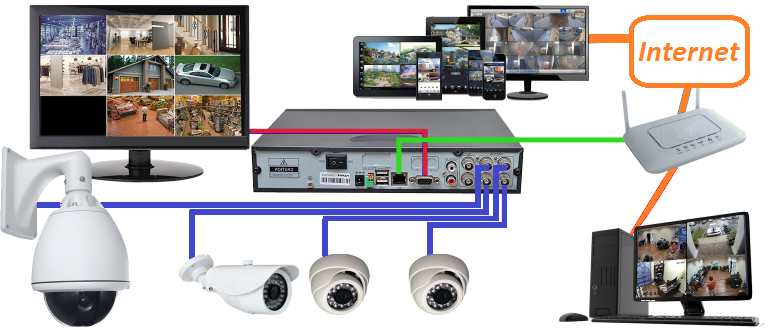
\includegraphics[width=9cm]{img/capitulo_2/sis_videovigilancia.png}
    \end{center}
    \caption{Sistema actual de videovigilancia\\Fuente: Web}
    \label{fig:sistema_video_vigilancia}
\end{figure}

La creciente demanda en el mercado de la vigilancia ha reducido costos en este tipo de sistemas, lo cual permitió que desarrolladores y fabricantes diseñen nuevas implementaciones de sistemas de video vigilancia agregándoles diversas capacidades dependiendo de la tecnología utilizada en su desarrollo. En la figura \ref{fig:surveillance-market} se muestra como el mercado global de la video vigilacia fue avaluado en 42.9 billones de dólares en 2019 y esta proyectado alcanzar a los 69.1 billones billones de dólares hasta el 2026, registrando una taza de crecimiento anual compuesta del 10\% desde el 2020 al 2026. \cite{marketsandmarkets:market-surveillance}\\

\begin{figure}[H]
    \begin{center}
        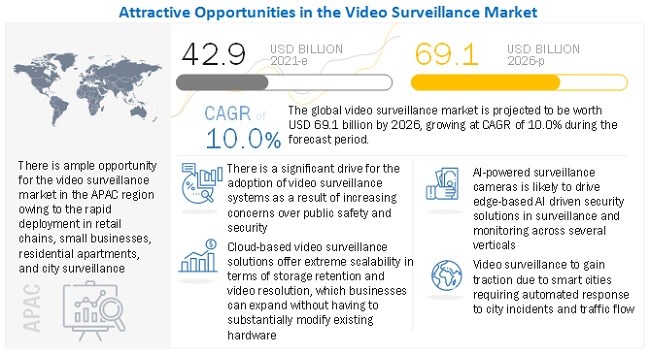
\includegraphics[width=13cm]{img/capitulo_2/surveillance-market.jpg}
    \end{center}
    \caption{Proyección del mercado de la videovigilancia\\Fuente: MarketsAndMarkets(web)}
    \label{fig:surveillance-market}
\end{figure}

El aspecto más importante a resaltar en el mercado de la videovigilancia es la potenciación de funcionalidades de estos sistemas gracias a la Inteligencia Artificial (I.A.) y la escalabilidad por servicios basados en la nube.Las técnicas de la inteligencia de artificial que potencian las utilidades de la videovigilancia son: visión por computadora, redes neuronales convolucionales, Machine Learning, Deep Learning, reconocimiento de patrones. (A completar segun bibliografia)\\

Para el desarrollo del prototipo propuesto se implementan todos los componentes involucrados en el sistema de videovigilancia como ser:
\begin{itemize}
    \item Cámaras (Nodos)
    \item Servidor TCP
    \item Servidor Web
    \item Aplicación Movil (Cliente)
\end{itemize}

A continuación se detalla los componentes que forman parte del prototipo del sistema de video vigilancia inteligente propuesto.

\section{Inteligencia Artificial}
La Inteligencia Artificial (I.A.), es una tecnología innovadora que en los últimos tiempos no esta reservado solo para la investigación sino más bien va tomando parte en el desarrollo de la sociedad. El cerebro es el órgano más increible del cuerpo humano; establece la forma en la que percibimos las imágenes, sonido, olores, sabores y el tacto. Nos permite almacenar recuerdos, experimentar emociones e incluso soñar. Sin él, los seres humanos serían organismos primitivos, incapaces de otra cosa que el más simple de los reflejos. Por lo tanto el cerebro es lo que hace a los seres humanos, seres inteligentes.\\

Durante décadas se ha investigado para construir máquinas inteligentes con cerebros como el del ser humano; asistentes robotizados para limpiar los hogares, coches que se conducen por solos, microscopios que detecten enfermedades automáticamente. Pero en la construcción de estas máquinas artificialmente inteligentes se presentan problemas computacionales complejos; problemas que el cerebro humano puede resolver en una fracción de segundos. Las formas de analizar y resolver este tipo de problemas, es el campo de estudio de la Inteligencia Artificial.

\section{Visión por Computadora}
La visión por computadora es una técnica de recolección de información que surge por la inspiración en el sistema visual humano, el cual es la principal fuente de información para el cerebro. Su meta es de modelar y automatizar el proceso de reconocimiento visual de objetos en la vida real.\\

De los cinco sentidos que poseen las personas, la vista es la más importante. Por lo tanto la visión, es una tarea de procesamiento de información; pero tiene un grado de complejidad elevado, ya que para saber que es lo qué hay en el mundo nuestros cerebros deben ser capaces de representar esta información en toda su abundancia de color, forma, movimiento, detalle y belleza. \cite{iaarbook:artificialvision}\\

Por lo tanto, la visión por computadora o visión artificial compone de un conjunto de herramientas y métodos que permiten obtener, procesar y analizar imágenes del mundo real, con el objetivo de ser tratadas por una computadora. Estos métodos van a permitir automatizar un amplio conjunto de tareas al aportar a las computadoras información que es necesaria para la toma de desiciones en sus tareas asignadas. La visión por computadora trata de imitar a la visión humana, usando geometría y un enfoque estadístico para tratar el problema.\\

\subsection{Aplicaciones}
Esta rama de la Inteligencia Artificial aún sigue en investigación y mejoras donde sus aplicaciones más comunes son:

\begin{itemize}
    \item \textbf{Reconocimiento óptico de caracteres:} Detección automática de símbolos que pertenecen a un alfabeto.
    \item \textbf{Inspección robotizada:} Revisión rápida de piezas para garantizar la calidad de componentes fabricados.
    \item \textbf{Modelado 3D:} Construcción de modelos 3D a partir de fotografías.
    \item \textbf{Imágenes médicas:} Análisis de radiografías.
    \item \textbf{Conducción segura:} Detección de obstáculos por medio de un sistema de conducción asistida por cámaras.
    \item \textbf{Vigilancia:} Monitoreo de intrusos, análisis del tráfico vial, monitoreo de piscinas, etc.
    \item \textbf{Detección de rostros:} Mediante algoritmos de reconocimiento facial se reconocen rostros usados en métodos de biometría.
\end{itemize}

\subsection{OpenCV}
Es una biblioteca de uso libre para el desarrollo de aplicaciones usando visión artificial desarrollada por Intel. Esta libreria reune diversas caracteristicas que la hacen popular, por ejemplo: 
\begin{itemize}
    \item Permite su uso para fines comerciales y de investigación.
    \item Se encuentra disponible par varias plataformas como ser GNU/Linux, Mac OS, Windows y Android.
    \item Documentación completa y explicada, con una comunidad de desarrolladores activa.
\end{itemize}

\begin{figure}[H]
    \begin{center}
        
\includegraphics[width=3cm]{img/capitulo_2/cv2_logo.png}
    \end{center}
    \caption{Logotipo de la libreria\\Fuente: Web}
    \label{fig:cv2_logo}
\end{figure}

Esta biblioteca permite:
\begin{itemize}
    \item El procesamiento de imágenes en su escalado, eliminación de ruido y formateo de imagen y video.
    \item El uso y modificación de sus 2500 modelos pre-optimizados que son incluidos en la libreria, acorde a las necesidades del usuario.
    \item El uso del estado del arte de modelos de visión por computadora como también de aprendizaje de máquina (Machine Learning).
    \item El desarrollo de modelos en varias categorías de investigación como ser: reconocimiento facial, detección y seguimiento de objetos, extracción de modelos 3D, etc.
\end{itemize}

Una de las características mas interesantes de OpenCV es el reconocimiento facial. OpenCV, en su extensa biblioteca de funciones, brinda las capacidades para realizar las tareas de preprocesamiento sin ningún problema, así como los algoritmos de predicción. Además de usar el algoritmo de detección de objetos, es posible usar el seguimiento de objetos, para identificar rostros en una transmisión de video. OpenCV incluso posee funciones para configurar fácilmente el modelo en una transmisión en vivo, como en un video pregrabado \cite{medium:opencv}. 

% \section{Redes Neuronales}

\section{Machine Learning}
Es un subcampo de la inteligencia artificial cuyo objetivo es entender la estructura de la información y ajustar estos datos en modelos que puedan ser entendidos y utilizados por las personas.\\

A diferencia de la computación tradicional, donde los algoritmos son grupos de instrucciones programadas ejecutadas por computadoras para resolver problemas específicos, los algoritmos de Machine Learning entrenan a las computadoras con datos de entrada y usa análisis estadístico para generar valores de salida que caen en un rango específico. Por eso el Machine Learning facilita a las computadoras construir modelos desde datos de ejemplo para automatizar el proceso de toma de decisiones basados en datos de entrada.\\

\subsection{Métodos de Machine Learning}
En el Machine Learning, las tareas son generalmente clasificadas en amplias categorias, las cuales estan basadas en como el aprendizaje es recibido o como la retroalimentación en el aprendizaje esta dado en un sistema desarrollado.\\

Dos de los más ampliamente adoptados de metodos en Machine Learning son el aprendizaje supervisado, que entrena un algoritmo basado en un ejemplo de entrada y salida que esta categorizada por un humano, y el aprendizaje no supervisado, que proporciona el algoritmo sin ningún dato categorizado para permitirle encontrar una estructura dentro de los datos de entrada.\\

\subsubsection{Aprendizaje Supervisado}
En lenguaje supervisado, la computadora esta provista con entradas de ejemplo que estan categorizados con sus salidas esperadas. El proposito de este metodo esta para que el algoritmo pueda "aprender" comparando la actual salida con las ``pensadas'' salidas para encontrar errores y en consecuencia modificar el modelo. El Aprendizaje supervisado por lo tanto usa patrones para predecir valores categorizados en datos no cateogirzados adicionales.\\

Por ejemplo, con aprendizaje supervisado, un algoritmo puede ser alimentado con imagenes de tiburones etiquetados como ``peces'' e imagenes de oceanos etiquetados como agua. Siendo entrenado con estso datos, el algoritmo de aprenizaje supervisado deberia poder despues identificar tiburones sin etiquetar como ``peces'' y oceanos no etiquetados como``agua''.\\

Un uso comun del aprendizaje supervisado es usar datos historicos para predecir estadsiticamente futuros eventos. Se puede usar la informacion historica del stock de un mercado para anticipar futuras fluctuaciones o ser empleado para filtrar correos fraudulentos. En aprendizaje supervisado, fotos de perros etiquetados pueden ser usados como datos de entradas para clasificar fotos de perros no etiquetados.\\

\subsubsection{Aprendizaje No Supervisado}
En el aprendizaje no supervisado, la informacion no esta categorizada, asi que los algoritmos de aprendizaje quedan para encontrar similitudes entre los datos de entrada. Como los datos no etiquetados son mas abundantes que los datos etiquetados. los metodos de ML que facilitan el aprendizaje no supervisado son particularmente valiosos.\\

El objetivo del aprendizaje no supervisado puede ser tan sencillo como descubrir patrones ocultos dentro de set de datos, pero esto puede tambien tener un objetivo de caracteristica de aprendizaje, que permite a la maquina computacional descubrir automaticamente las represetnaciones que son necesarias para clasificar datos en bruto.\\

Aprendizaje no supervisado es comunmente usado para datos transaccionales. Puedes tener un dataset grande de clientes y sus compras, pero como humano probablemente no podras tener sentido de que atributos similares pueden ser dibujados de los perfiles de los clientes y sus tipos de compras. Con esta informacion se alimenta un algoritmo de aprendizaje no supervisado, esto podria determinar que las mujeres de cierto rango de edad quienes compran jabones sin olor estan probablemente embarazadas, and por lo tanto una campania de marketing relacionada con el embarazo y productos para bebé pueden ser etiquetados para esta audiencia con el objetivo de incrementar el numero de compras.\\

\section{Protocolos de red}

\subsection{TCP/IP}

\subsection{HTTP}

\section{Video Streaming}

\subsection{Formatos}

\subsubsection{HLS}

\subsubsection{DASH}

\section{Aplicaciones Móviles}

\subsection{Android}

\subsection{Firebase}

\subsection{Exoplayer}

\section{Python}
Python es un lenguaje de programación interpretado cuya filosofía hace hincapié en la legibilidad de su código. Se trata de un lenguaje multiparadigma, ya que soporta parcialmente la orientación a objetos, programación imperativa y, en menor medida, programación funcional. Es un lenguaje interpretado, dinámico y multiplataforma.\\

Python usa tipado dinámico y conteo de referencias para la administración de memoria. Una característica importante de Python es la resolución dinámica de nombres; es decir, lo que enlaza un método y un nombre de variable durante la ejecución del programa (también llamado enlace dinámico de métodos).\\

\section{Metodología de desarrollo Cascada}